% n9n research paper. Built with pdflatex + IEEEtran (conference mode).
% Drafted 2026-10-23 by Claude Fable 5.1 (claude-fable-5-1) for the n9n project; see paper/README.md.
\documentclass[conference]{IEEEtran}
\usepackage[utf8]{inputenc}
\usepackage[T1]{fontenc}
\usepackage{cite}
\usepackage{amsmath}
\usepackage{graphicx}
\usepackage{booktabs}
\usepackage{array}
\usepackage{url}
\usepackage{xcolor}
\usepackage{tikz}
\usetikzlibrary{arrows.meta,positioning,shapes.geometric,calc,fit}
\usepackage[hidelinks]{hyperref}
\renewcommand{\arraystretch}{1.15}
\renewcommand{\ttdefault}{cmtt}
\newcolumntype{L}[1]{>{\raggedright\arraybackslash}p{#1}}
\IEEEoverridecommandlockouts
\renewcommand{\topfraction}{0.95}\renewcommand{\bottomfraction}{0.9}\renewcommand{\textfraction}{0.05}\renewcommand{\floatpagefraction}{0.75}\setcounter{topnumber}{4}\setcounter{bottomnumber}{3}\setcounter{totalnumber}{6}\setcounter{dbltopnumber}{2}

\begin{document}
\newcommand{\LATn}{50}
\newcommand{\LATmedian}{260}
\newcommand{\LATpNN}{290}
\newcommand{\LATstepsum}{7}
\newcommand{\THRone}{71.3}
\newcommand{\THRfour}{178.5}
\newcommand{\THReight}{158.6}
\newcommand{\THRn}{100}
\newcommand{\THRenq}{0.1}
\newcommand{\THRbest}{178.5}
\newcommand{\REPreps}{10}
\newcommand{\REPcopy}{5}
\newcommand{\REPexec}{4}
\newcommand{\FAULTrecover}{0.3}


\title{AI Workflow using Agentic Orchestration and SEO}

\author{
\IEEEauthorblockN{Anmol Bhardwaj}
\IEEEauthorblockA{Dept. of Computer Science and\\Engineering (AI/ML)\\Meerut Institute of Engineering\\and Technology (MIET), Meerut\\Dr. A P J Abdul Kalam Technical\\University (AKTU), Uttar Pradesh, India}
\and
\IEEEauthorblockN{Avi Gupta}
\IEEEauthorblockA{Dept. of Computer Science and\\Engineering (AI/ML)\\Meerut Institute of Engineering\\and Technology (MIET), Meerut\\Dr. A P J Abdul Kalam Technical\\University (AKTU), Uttar Pradesh, India}
\and
\IEEEauthorblockN{Jatin Raghav}
\IEEEauthorblockA{Dept. of Computer Science and\\Engineering (AI/ML)\\Meerut Institute of Engineering\\and Technology (MIET), Meerut\\Dr. A P J Abdul Kalam Technical\\University (AKTU), Uttar Pradesh, India}
\and
\IEEEauthorblockN{Keshav Garg}
\IEEEauthorblockA{Dept. of Computer Science and\\Engineering (AI/ML)\\Meerut Institute of Engineering\\and Technology (MIET), Meerut\\Dr. A P J Abdul Kalam Technical\\University (AKTU), Uttar Pradesh, India}
}

\maketitle

\begin{abstract}
Rule-based workflow platforms such as Zapier, Make, n8n and Node-RED execute fixed trigger--action chains reliably but cannot interpret context or recover from states they were not programmed for. Large language model (LLM) agents can reason, plan and call tools, but benchmark studies show that they remain unreliable on open-ended tasks and that their execution is neither reproducible nor auditable. This paper studies how the two paradigms can be combined into one production-oriented platform, with search engine optimisation (SEO) auditing as the application domain. We review twenty-two works on reasoning-and-acting loops, tool use, multi-agent coordination, agent evaluation and generative engine optimisation, compare them on the properties a production workflow engine needs, and identify the gap: no reviewed system provides durable, replayable, side-effect-safe execution as the substrate on which agentic decisions are made. We then present n9n, a hybrid platform whose deterministic substrate (a Go API, a Rust worker and PostgreSQL) is implemented, and whose agentic layer (a prompt-to-workflow builder with a validate-and-repair loop, and a run-failure explainer with a code-enforced retry rule) and SEO layer are specified on top of it. The substrate is evaluated on a local deployment: a seven-node branching workflow completes in a median of \LATmedian{} ms end to end with \LATstepsum{} ms of recorded step time; a burst of 100 runs sustains \THRone{}, \THRfour{} and \THReight{} runs/s at worker concurrency 1, 4 and 8; replaying a nine-node run from its sixth node re-executes only \REPexec{} steps and reuses \REPcopy{}; a technical SEO audit workflow built from existing nodes classifies status, redirect, retry and missing-title cases correctly; and a worker killed during a side-effecting step is recovered as \emph{queued} and completed when the step is idempotent, and marked \emph{uncertain} when it is not, with the verdict recorded \FAULTrecover{} s after the lease expires. These results characterise the substrate only; the agentic and SEO reasoning components are not yet measured, and an evaluation plan for them is given.
\end{abstract}

\begin{IEEEkeywords}
agentic AI, workflow orchestration, large language models, multi-agent systems, durable execution, replay, SEO automation, generative engine optimisation, Go, Rust
\end{IEEEkeywords}

\section{Introduction}
Workflow automation has historically relied on rigid, event-triggered rule chains: a trigger fires, a condition is checked and a predefined action executes. This model, popularised by Zapier, Make, n8n and Node-RED, suits repetitive, well-specified integration tasks but breaks down when a workflow must interpret ambiguous content, weigh alternatives or recover from an unexpected state. Large language models that can reason, plan and invoke external tools offer an alternative: \emph{agentic} systems in which a model analyses a situation, decides on an action and executes it, possibly with other agents \cite{yao2023react,wu2023autogen}.

The two paradigms have complementary weaknesses. Rule engines are predictable and auditable but cannot decide. Agents can decide but, as WebArena, AgentBench and GAIA show \cite{zhou2024webarena,liu2024agentbench,mialon2023gaia}, they succeed on a minority of realistic tasks, are sensitive to prompt and model changes, and leave no execution record that a person can replay. A production system that uses an agent for a judgement call therefore needs a substrate that makes the deterministic parts of a workflow durable, replayable and safe against duplicated side effects, so that the agent's unreliability is contained rather than amplified.

This paper takes SEO auditing as the application domain. Technical SEO checks (reachability, status codes, redirects, robots and sitemap files, title and metadata presence) are deterministic and should never be delegated to a model; content assessments (relevance, intent match, readability) are judgement calls that a model can make. Recent work on generative engine optimisation (GEO) \cite{aggarwal2024geo} shows that visibility in LLM-driven search is itself becoming an optimisation target, which makes an automation platform that can combine fixed checks with model judgement timely.

The paper makes five contributions:
\begin{enumerate}
\item a structured review of twenty-two works on reasoning-and-acting, tool use, multi-agent coordination, agent evaluation and GEO, each with its limitation for production workflow use;
\item a comparative analysis and a research gap centred on the absence of a durable, replayable substrate beneath agentic decisions;
\item the design of n9n, a three-layer platform: a deterministic substrate, an agentic layer and an SEO layer;
\item an implementation of the substrate (Go API, Rust worker, PostgreSQL, Flutter web and React Native clients) and its measured evaluation on latency, throughput, replay, fault recovery and a technical SEO audit workflow; and
\item an evaluation plan for the agentic and SEO layers, which are specified but not yet measured.
\end{enumerate}
Section~II states the review scope, Section~III reviews the works, Section~IV compares them and Section~V states the gap. Section~VI presents n9n, Section~VII maps it to the literature, Section~VIII reports the implementation and its evaluation, Section~IX gives limitations, Section~X the evaluation plan and Section~XI concludes.

\section{Review Scope and Priority}
The review covers twenty-two works selected for their relevance to running LLM decisions inside an automated workflow. Bibliographic details were checked against the arXiv record or the publisher page of each work; where a venue could not be confirmed from the record, the arXiv identifier is cited. The works fall into four strands, listed in the order of their importance to n9n:
\begin{itemize}
\item \textbf{Strand 1, single-agent reasoning and tool use:} ReAct, Toolformer, Plan-and-Solve, Tree of Thoughts, Reflexion, Self-Ask, CodeAct and Gorilla. These define how one model plans, acts and calls tools, which is what an agent node in a workflow does.
\item \textbf{Strand 2, multi-agent and orchestration frameworks:} AutoGen, CAMEL, MetaGPT, HuggingGPT, Voyager, and the platforms n8n and LangGraph. These define how several agents or steps are coordinated.
\item \textbf{Strand 3, evaluation:} WebArena, AgentBench, GAIA, $\tau$-bench and SWE-agent. These measure how reliable agents are and so bound how much autonomy a workflow should grant.
\item \textbf{Strand 4, SEO and surveys:} GEO, and the agent surveys of Wang et al., Xi et al. and Masterman et al., which frame the design space.
\end{itemize}

\section{Detailed Review}

\subsection{ReAct: Synergizing Reasoning and Acting}
Yao et al. \cite{yao2023react} interleave free-text reasoning traces with discrete actions so that reasoning can update a plan and decide when to query an external source, while actions return observations that feed later reasoning. On HotpotQA and FEVER the model queries a Wikipedia API; on ALFWorld and WebShop it outperforms imitation and reinforcement learning baselines by 34\% and 10\% absolute success. \emph{Limitation:} the loop is a single prompt-driven process with no persistence; if the process dies, the trajectory is lost, and the same input can take a different path on a second run. \emph{Relevance:} ReAct is the execution model of a single agent node; n9n wraps such a node in a step record so that its inputs, outputs and the branch it chose are stored like any other step.

\subsection{Toolformer}
Schick et al. \cite{schick2023toolformer} train a model, in a self-supervised way from a few demonstrations per API, to decide which tool to call, when and with what arguments, covering a calculator, question answering, two search engines, translation and a calendar. \emph{Limitation:} the tool set is fixed at training time, and the paper gives no mechanism for recording or retrying a call that has side effects. \emph{Relevance:} tool calling is how an agent node would invoke n9n's HTTP and email actions; the platform, not the model, records each attempt.

\subsection{Plan-and-Solve Prompting}
Wang et al. \cite{wang2023plansolve} first ask the model for a plan that divides the task into subtasks and then for their execution, reducing the missing-step errors of zero-shot chain-of-thought across ten datasets. \emph{Limitation:} the gains are shown on reasoning benchmarks; the plan is text and is not validated against an executable schema. \emph{Relevance:} n9n's workflow builder asks a model for a plan in the form of a graph and validates that graph with the same code that guards publishing.

\subsection{Tree of Thoughts}
Yao et al. \cite{yao2023tot} treat each reasoning step as a node in a search tree that the model explores, evaluates and backtracks over; on Game of 24, GPT-4 with chain-of-thought solved 4\% of instances and Tree of Thoughts 74\%. \emph{Limitation:} search multiplies model calls and cost, and the evaluation covers three puzzle-like tasks. \emph{Relevance:} search over candidate graphs is a possible extension of the builder's repair loop, but its cost argues for bounding it, as n9n does with a fixed number of repair rounds.

\subsection{Reflexion}
Shinn et al. \cite{shinn2023reflexion} reinforce agents through linguistic feedback rather than weight updates: the agent reflects on a failed trial, stores the reflection in an episodic memory and uses it in the next trial, reaching 91\% pass@1 on HumanEval. \emph{Limitation:} the method assumes trials can be repeated freely, which is false for workflows with side effects such as sending email. \emph{Relevance:} n9n's failure explainer is a one-shot, human-reviewed form of reflection; the platform forbids automatic retries of non-idempotent steps.

\subsection{Self-Ask and the Compositionality Gap}
Press et al. \cite{press2023selfask} define the compositionality gap, the fraction of compound questions a model fails although it answers each sub-question, and show that it does not shrink with model size in the GPT-3 family; self-ask prompting, which makes the model ask and answer follow-up questions, narrows it. \emph{Limitation:} the result is on question answering, and decomposition is left to the model. \emph{Relevance:} it motivates decomposing a workflow into explicit nodes rather than asking one agent to do everything.

\subsection{CodeAct}
Wang et al. \cite{wang2024codeact} unify an agent's action space as executable Python code run in an interpreter, reporting up to 20\% higher success than JSON or text actions across 17 models. \emph{Limitation:} arbitrary code execution requires sandboxing and makes the effect of an action hard to audit. \emph{Relevance:} n9n plans a sandboxed WebAssembly code node with no system capabilities, fuel and memory limits, and keeps it disabled by default.

\subsection{Gorilla}
Patil et al. \cite{patil2023gorilla} fine-tune a LLaMA model to write API calls and pair it with a document retriever so that it adapts to documentation changes at test time; APIBench is built from three model hubs. \emph{Limitation:} the scope is API-call synthesis, not execution, and hallucinated calls are still possible. \emph{Relevance:} n9n gives the model the node catalogue with configuration, input and output schemas, and rejects any generated graph that fails validation.

\subsection{AutoGen}
Wu et al. \cite{wu2023autogen} present an open-source framework in which customisable, conversable agents, backed by models, humans or tools, converse to complete a task, with interaction patterns defined in natural language and code. \emph{Limitation:} conversation state lives in process memory; the framework provides no durable log, replay or deduplication of side effects. \emph{Relevance:} AutoGen's human-in-the-loop agent corresponds to n9n's planned approval node, which pauses a run in the database until a person decides.

\subsection{CAMEL}
Li et al. \cite{li2023camel} propose role-playing between communicative agents guided by inception prompts, and use it to generate cooperation data. \emph{Limitation:} the framework studies agent societies rather than reliable task completion. \emph{Relevance:} role assignment informs how an SEO content agent and a verification agent could be separated.

\subsection{MetaGPT}
Hong et al. \cite{hong2023metagpt} encode standard operating procedures as prompt sequences and assign agents roles in an assembly line, so that intermediate results are verified and cascading hallucinations are reduced. \emph{Limitation:} the procedures are fixed in prompts and the evaluation is on software generation tasks. \emph{Relevance:} the idea that intermediate outputs are checked by a separate stage matches n9n's rule that every agent output passes a deterministic validator before it is used.

\subsection{HuggingGPT}
Shen et al. \cite{shen2023hugginggpt} use a chat model as a controller that plans tasks, selects models from a hub by their descriptions, runs them and summarises. \emph{Limitation:} planning quality depends on the controller, and failures in a selected model are not retried in a principled way. \emph{Relevance:} it is an early example of an LLM planning over a catalogue of tools, which is what the n9n builder does over node types.

\subsection{Voyager}
Wang et al. \cite{wang2023voyager} sustain open-ended behaviour in Minecraft with an automatic curriculum, a library of skills stored as executable code and iterative prompting driven by execution errors. \emph{Limitation:} the setting is a game with no side effects outside it. \emph{Relevance:} a published workflow version is a reusable skill; n9n stores versions immutably so a skill cannot change under a running job.

\subsection{n8n and LangGraph}
n8n \cite{n8n} is an open-source node-based automation platform with hundreds of integrations and an AI agent node; LangGraph \cite{langgraph} orchestrates stateful agent graphs with checkpointing and human-in-the-loop interrupts. \emph{Limitation:} both allow cycles and arbitrary code in nodes, which makes publish-time validation weak, and neither records per-request attempts or classifies an interrupted side effect as uncertain. \emph{Relevance:} they are the closest systems to n9n, which deliberately restricts the graph to a validated directed acyclic graph with one trigger.

\subsection{WebArena}
Zhou et al. \cite{zhou2024webarena} provide self-hosted, functional websites in four domains with tasks graded on functional correctness; the best GPT-4 agent reaches 14.41\% end-to-end success against 78.24\% for humans. \emph{Limitation:} the environment is web interaction only. \emph{Relevance:} it quantifies why an agent must not be given unsupervised control of side-effecting steps.

\subsection{AgentBench}
Liu et al. \cite{liu2024agentbench} evaluate models as agents in eight environments and attribute failures to poor long-term reasoning, decision-making and instruction following, with a large gap between commercial and open models. \emph{Limitation:} the benchmark measures models, not the systems around them. \emph{Relevance:} it supports choosing a model per deployment through configuration rather than hard-coding one.

\subsection{GAIA}
Mialon et al. \cite{mialon2023gaia} pose 466 real-world assistant questions that need reasoning, browsing and tool use; humans score 92\% and GPT-4 with plugins 15\%. \emph{Limitation:} answers to 300 questions are withheld, so local evaluation is partial. \emph{Relevance:} it motivates keeping deterministic checks deterministic.

\subsection{$\tau$-bench}
Yao et al. \cite{yao2024taubench} simulate conversations between a user model and a tool-using agent under policy constraints, score success by the final database state and introduce pass\^{}k for reliability over repeated trials; GPT-4o passes fewer than half the tasks and has pass\^{}8 below 25\% in retail. \emph{Limitation:} the user is simulated. \emph{Relevance:} pass\^{}k is the metric n9n adopts for its agentic components, and database-state checking matches n9n's recorded step outputs.

\subsection{SWE-agent}
Yang et al. \cite{yang2024sweagent} show that an agent--computer interface designed for a model, with constrained file and repository commands, changes agent behaviour and reaches 12.5\% pass@1 on SWE-bench. \emph{Limitation:} the interface is specific to software repositories. \emph{Relevance:} it argues that the interface offered to an agent should be narrow and typed, as n9n's node catalogue is.

\subsection{GEO: Generative Engine Optimization}
Aggarwal et al. \cite{aggarwal2024geo} formalise generative engines, propose a black-box framework for raising a source's visibility in generated answers and release GEO-bench; the best strategies raise visibility by up to 40\%, but efficacy varies by domain. \emph{Limitation:} the work optimises content for visibility and does not address auditing a site's technical health. \emph{Relevance:} it defines the content-side SEO tasks that n9n's agent nodes would perform, after deterministic technical checks pass.

\subsection{Surveys}
Wang et al. \cite{wang2024survey} propose a unified construction framework for LLM agents and review applications and evaluation; Xi et al. \cite{xi2023rise} frame agents as brain, perception and action, and discuss single-agent, multi-agent and human--agent settings; Masterman et al. \cite{masterman2024landscape} compare single- and multi-agent architectures and discuss leadership and communication styles. \emph{Limitation:} as surveys they name open problems rather than solving them. \emph{Relevance:} all three list reliability, evaluation and safe tool use as open, which is the gap this paper addresses from the systems side.

\section{Comparative Analysis}
Table~\ref{tab:compare} compares the reviewed works on the properties a production workflow substrate needs: whether execution state is durable, whether a run can be replayed from a step, whether side effects are protected against duplication, and whether outputs are validated by code before use. The columns are judged from each work's own description; a dash means the work does not address the property, which is not a criticism of its goals.

\begin{table*}[!t]
\centering
\caption{Comparative Analysis of Reviewed Works}
\label{tab:compare}
\small
\begin{tabular}{L{2.3cm} L{1.5cm} L{3.4cm} L{1.4cm} L{1.3cm} L{1.7cm} L{3.3cm}}
\toprule
\textbf{Work} & \textbf{Strand} & \textbf{Main contribution} & \textbf{Durable state} & \textbf{Replay} & \textbf{Side-effect safety} & \textbf{n9n use} \\
\midrule
ReAct \cite{yao2023react} & Single agent & Interleaved reasoning and acting & -- & -- & -- & Execution model of an agent node \\
Toolformer \cite{schick2023toolformer} & Single agent & Self-supervised tool calling & -- & -- & -- & Tool calls become HTTP/email steps \\
Plan-and-Solve \cite{wang2023plansolve} & Single agent & Plan before execution & -- & -- & -- & Builder plans a graph, then it is validated \\
Tree of Thoughts \cite{yao2023tot} & Single agent & Search over reasoning steps & -- & -- & -- & Bounded repair rounds instead of open search \\
Reflexion \cite{shinn2023reflexion} & Single agent & Verbal self-reflection across trials & Episodic memory (in process) & -- & -- & One-shot failure explainer, human reviewed \\
Self-Ask \cite{press2023selfask} & Single agent & Decomposition into sub-questions & -- & -- & -- & Explicit nodes rather than one agent \\
CodeAct \cite{wang2024codeact} & Single agent & Code as the action space & -- & -- & -- & Sandboxed code node, off by default \\
Gorilla \cite{patil2023gorilla} & Single agent & API-call synthesis with retrieval & -- & -- & -- & Catalogue schemas in the builder prompt \\
AutoGen \cite{wu2023autogen} & Multi-agent & Conversable agents incl. humans & -- & -- & -- & Approval node as human agent \\
CAMEL \cite{li2023camel} & Multi-agent & Role-playing agents & -- & -- & -- & Separate content and verification roles \\
MetaGPT \cite{hong2023metagpt} & Multi-agent & SOPs and verified intermediates & -- & -- & -- & Validator between agent and use \\
HuggingGPT \cite{shen2023hugginggpt} & Multi-agent & LLM controller over a model hub & -- & -- & -- & Planning over a node catalogue \\
Voyager \cite{wang2023voyager} & Multi-agent & Skill library, curriculum & Skill library & -- & -- & Immutable workflow versions as skills \\
n8n \cite{n8n} & Platform & Node-based automation with AI node & Yes & Partial (re-run) & -- & Closest product; n9n restricts graphs \\
LangGraph \cite{langgraph} & Platform & Stateful agent graphs, checkpoints & Yes & From checkpoint & -- & Checkpointing; n9n adds uncertain state \\
WebArena \cite{zhou2024webarena} & Evaluation & Functional web tasks & -- & -- & -- & Bounds autonomy of agent nodes \\
AgentBench \cite{liu2024agentbench} & Evaluation & Eight-environment benchmark & -- & -- & -- & Model chosen by configuration \\
GAIA \cite{mialon2023gaia} & Evaluation & Real assistant questions & -- & -- & -- & Keep deterministic checks deterministic \\
$\tau$-bench \cite{yao2024taubench} & Evaluation & State-based scoring, pass\^{}k & -- & -- & -- & Metric for the agentic layer \\
SWE-agent \cite{yang2024sweagent} & Evaluation & Agent--computer interface design & -- & -- & -- & Narrow, typed node interface \\
GEO \cite{aggarwal2024geo} & SEO & Visibility in generative engines & -- & -- & -- & Content tasks for agent nodes \\
Surveys \cite{wang2024survey,xi2023rise,masterman2024landscape} & Survey & Design space, open problems & -- & -- & -- & Framing of the gap \\
\bottomrule
\end{tabular}
\end{table*}

\section{Research Gap}
The reviewed literature gives a mature account of how a single model reasons and calls tools, several ways to coordinate many agents, and increasingly realistic benchmarks that show those agents succeeding on a minority of open-ended tasks. What it does not give is the systems layer that a production workflow needs around those agents:
\begin{itemize}
\item \textbf{No durable, replayable execution record.} ReAct-style loops and conversation frameworks keep state in process memory. LangGraph checkpoints state, but no reviewed work lets a person re-run a finished run from a chosen step with edited input while reusing the recorded upstream outputs.
\item \textbf{No treatment of interrupted side effects.} None of the works distinguishes a step that may be retried from one whose effect is unknown after a crash. Reflexion and Tree of Thoughts assume trials are free to repeat.
\item \textbf{Validation of agent output is left to the model.} Plan-and-Solve and HuggingGPT trust the generated plan; Gorilla reduces but does not eliminate hallucinated calls. No work routes a generated artefact through the same validator that guards human-authored ones.
\item \textbf{Deterministic and agentic steps are not separated by design.} Benchmarks show agents fail on tasks a rule would solve, yet frameworks let an agent own the whole task.
\item \textbf{SEO is treated as content optimisation only.} GEO addresses visibility in generative engines; no reviewed work combines deterministic technical audits with model-based content assessment in one automated workflow.
\item \textbf{Reliability is rarely measured over repeated trials.} $\tau$-bench's pass\^{}k is the exception; platform papers report single-run success.
\end{itemize}
n9n addresses the first four gaps with an implemented substrate, and the last two with a specified design and an evaluation plan.

\section{Proposed System: n9n}
n9n is a visual workflow automation platform organised in three layers (Fig.~\ref{fig:arch}). The \emph{deterministic substrate} stores, validates, versions and executes workflows and is implemented. The \emph{agentic layer} adds model-driven construction and diagnosis of workflows and, as a later step, agent nodes inside them; it is specified in the project's platform plan and gated behind configuration. The \emph{SEO layer} is an application of both: technical checks are ordinary deterministic nodes, and content assessment is an agent node.

\begin{figure}[!htbp]
\centering
\resizebox{\columnwidth}{!}{%
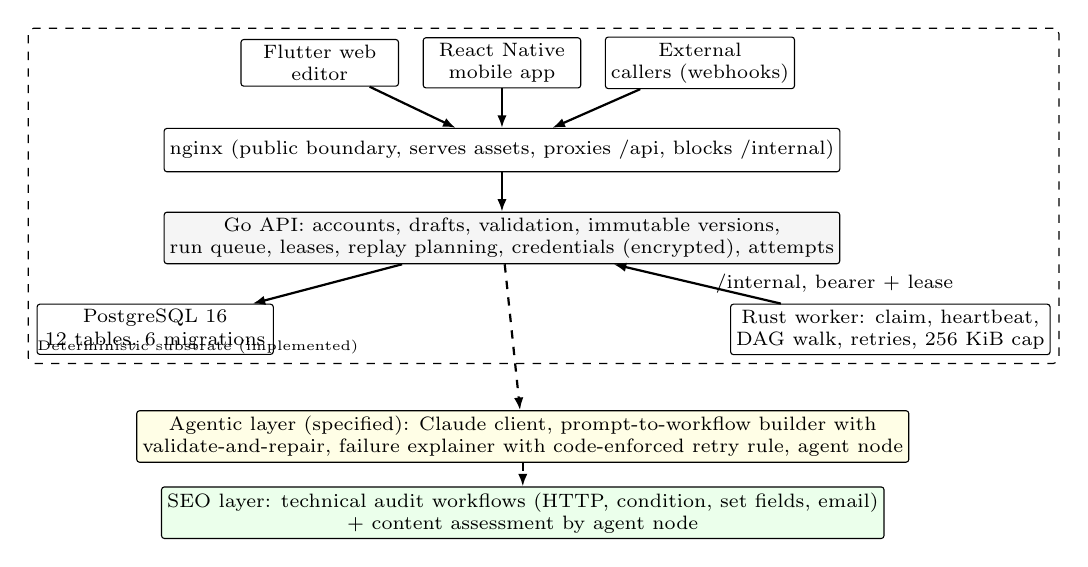
\begin{tikzpicture}[font=\scriptsize, node distance=3mm,
  box/.style={draw, rounded corners=1pt, minimum height=5.5mm, inner sep=2pt, align=center},
  layer/.style={draw, dashed, rounded corners=2pt, inner sep=3pt},
  arr/.style={-{Latex[length=1.6mm]}, thick}]
\node[box, minimum width=20mm] (web) {Flutter web\\editor};
\node[box, minimum width=20mm, right=of web] (mob) {React Native\\mobile app};
\node[box, minimum width=20mm, right=of mob] (hook) {External\\callers (webhooks)};
\node[box, minimum width=66mm, below=5mm of mob] (nginx) {nginx (public boundary, serves assets, proxies /api, blocks /internal)};
\node[box, minimum width=66mm, below=5mm of nginx, fill=gray!8] (api) {Go API: accounts, drafts, validation, immutable versions,\\run queue, leases, replay planning, credentials (encrypted), attempts};
\node[box, minimum width=30mm, below left=5mm and -14mm of api] (pg) {PostgreSQL 16\\12 tables, 6 migrations};
\node[box, minimum width=30mm, below right=5mm and -14mm of api] (runner) {Rust worker: claim, heartbeat,\\DAG walk, retries, 256 KiB cap};
\node[box, minimum width=66mm, anchor=north, fill=yellow!10] at ($(pg.south)!0.5!(runner.south)+(0,-7mm)$) (ai) {Agentic layer (specified): Claude client, prompt-to-workflow builder with\\validate-and-repair, failure explainer with code-enforced retry rule, agent node};
\node[box, minimum width=66mm, below=3mm of ai, fill=green!8] (seo) {SEO layer: technical audit workflows (HTTP, condition, set fields, email)\\+ content assessment by agent node};
\draw[arr] (web) -- (nginx); \draw[arr] (mob) -- (nginx); \draw[arr] (hook) -- (nginx);
\draw[arr] (nginx) -- (api);
\draw[arr] (api) -- (pg); \draw[arr] (runner) -- node[right, xshift=1mm]{/internal, bearer + lease} (api);
\draw[arr, dashed] (api) -- (ai);
\draw[arr, dashed] (ai) -- (seo);
\node[layer, fit=(web)(hook)(nginx)(api)(pg)(runner), label={[anchor=south west]south west:\tiny Deterministic substrate (implemented)}] {};
\end{tikzpicture}}
\caption{Three-layer architecture of n9n. Solid boxes are implemented; the agentic layer is specified and feature-flagged (\texttt{GET /api/features} reports \texttt{ai:false} until a model key is configured).}
\label{fig:arch}
\end{figure}

\subsection{Deterministic Substrate}
\subsubsection{Workflow model}
A workflow is a directed acyclic graph of typed nodes. Publishing validates that the graph has exactly one trigger, that every action has at most one incoming edge, that every node is reachable from the trigger, that there is no cycle, and that every configuration field and \texttt{\{\{input.x\}\}} or \texttt{\{\{nodes.ID.x\}\}} mapping refers to a node that is an ancestor. The node catalogue (version 2) has eight types: manual, webhook, schedule and Gmail triggers; set-fields, HTTP request, condition and send-email actions. Only \texttt{condition} has \texttt{true} and \texttt{false} output ports. Publishing snapshots the graph as an immutable numbered version; a draft edit never changes a queued or running job. A draft can also be executed as a \emph{test} run against a snapshot stored on the run record without publishing.

\subsubsection{Durable queue and leases}
Runs are rows in PostgreSQL. A worker claims the oldest queued run with a row lock and \texttt{SKIP LOCKED}, so several workers can share one database, and receives a 60-second lease that it extends every 10 seconds by heartbeat. Every step reports its status, input, output, branch, attempt number and timing to the API, so the database holds the full execution trace. If a lease expires, the next claim examines the steps that were running or failed: if any belongs to a send-email node, or to an HTTP node whose method is not GET or HEAD and that has no idempotency key, the run is marked \emph{uncertain} with the reason recorded; otherwise it is re-queued and resumed, reusing every step that already succeeded. A cancelled run fences the old lease so a late worker cannot write to it.

\subsubsection{Attempts, limits and isolation}
GET, HEAD and idempotent HTTP requests are retried up to three times on a 5xx response or transport failure; every request, including retries, is recorded as an attempt with status, error and duration, scoped to the execution attempt of its step. Redirects are not followed, so a 301 is reported as such. Destinations must resolve to public addresses unless the operator allows private ones. Step outputs are capped at 256 KiB, JSON nesting at 32 levels and public requests at 1 MiB. Gmail secrets are encrypted at rest with a server-side key and are never returned to clients. Browser sessions use an HttpOnly cookie; mobile clients use revocable bearer tokens; webhook events are deduplicated by event identifier with tombstones that survive run retention.

\subsubsection{Replay}
A finished run can be replayed from any node, with an optional input override, against its original graph or the current draft. The API walks the graph from the trigger the way the worker will: conditions on the path to the chosen node are forced onto that path, other conditions keep their recorded branch, and only reached nodes that succeeded in the parent are copied as succeeded steps. A node that never completed in the parent is rejected rather than silently re-sent. The replay is a new run of kind \texttt{replay} linked to its parent, so the lineage is queryable.

\subsection{Agentic Layer}
The platform plan specifies the agentic layer in detail; it is summarised here because the evaluation plan in Section~X depends on it. All model calls go through one client in the Go API, are off unless an API key is configured, are rate-limited per user (30 requests per hour by default), and are logged with token counts. Workflow graphs may be sent to the model; run inputs and outputs are sent only if the operator enables it and the user confirms per request; credential values, webhook secrets and HTTP header values are redacted before any prompt is built, and a unit test fails if a known secret appears in an outgoing request.

\subsubsection{Prompt-to-workflow builder}
Given a sentence, the model receives the node catalogue with its schemas, the user's credential names and the mapping syntax, and returns a graph in the draft format. The API runs the same publish validator on the proposal; on failure it returns the errors to the model and asks for a corrected graph, up to three rounds. Only a validated graph reaches the editor, as an unsaved draft the user can test before publishing. This is Plan-and-Solve with a code validator in place of the model's own judgement.

\subsubsection{Failure explainer}
For a failed or uncertain run, the model receives the graph snapshot, the failing step, prior steps subject to the data policy, the recorded attempts and the documentation of the node types involved, and returns a summary, a likely cause, a \texttt{safe\_to\_retry} verdict and an optional graph patch. The verdict is overridden in code to \emph{no} for any uncertain run whose unsafe node lacks an idempotency key. A proposed fix can be applied to the draft or tested through replay-against-draft with the failed run's input, so the user sees it work before publishing. This is a single, human-reviewed Reflexion step.

\subsubsection{Agent node}
An agent node, planned after the builder and explainer, would execute a ReAct loop whose tools are the existing node actions, with its reasoning trace stored as the step's output and its tool calls recorded as attempts. Because it may call side-effecting tools, it is classified unsafe for lease recovery, like send-email.

\subsection{SEO Layer}
Technical SEO auditing decomposes into checks that have exact answers: a page is reachable or not, returns 200 or not, redirects or not, has a title tag or not, and serves \texttt{robots.txt} and a sitemap or not. Fig.~\ref{fig:seo} shows the audit workflow used in Section~VIII, built from existing nodes only: a webhook trigger receives a URL, an HTTP node fetches it, a condition on the body separates pages without a title, and set-fields nodes record a verdict; a page that is unreachable or answers with a non-2xx status fails the fetch step, and the status is read from the recorded attempt. Because the HTTP node records attempts, a page that fails twice and then succeeds is reported with three attempts rather than as a failure, and a redirect is reported as its status code rather than silently followed. Content assessment (relevance to a target query, intent match, readability, and the GEO-style visibility strategies of \cite{aggarwal2024geo}) is where an agent node is used, after the deterministic checks pass, so that a model never decides whether a page exists.

\begin{figure}[!htbp]
\centering
\resizebox{\columnwidth}{!}{%
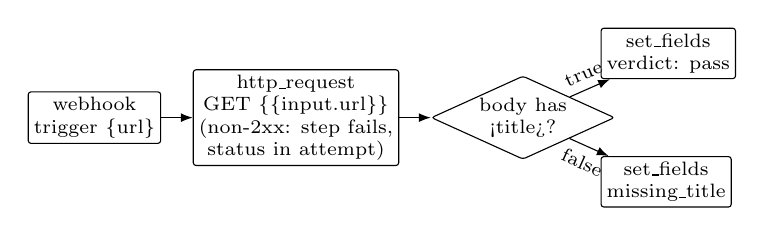
\begin{tikzpicture}[font=\scriptsize, node distance=2.2mm and 4mm,
  n/.style={draw, rounded corners=1pt, minimum height=5mm, inner sep=2pt, align=center},
  c/.style={n, diamond, aspect=2.2, inner sep=0.5pt},
  arr/.style={-{Latex[length=1.5mm]}}]
\node[n] (t) {webhook\\trigger \{url\}};
\node[n, right=of t] (f) {http\_request\\GET \{\{input.url\}\}\\(non-2xx: step fails,\\status in attempt)};
\node[c, right=of f] (h) {body has\\<title>?};
\node[n, above right=of h] (p) {set\_fields\\verdict: pass};
\node[n, below right=of h] (nt) {set\_fields\\missing\_title};
\draw[arr] (t) -- (f); \draw[arr] (f) -- (h);
\draw[arr] (h) -- node[above, sloped]{true} (p); \draw[arr] (h) -- node[below, sloped]{false} (nt);
\end{tikzpicture}}
\caption{Technical SEO audit workflow built from existing n9n nodes (five nodes, four edges). A non-2xx response fails the fetch step with the status recorded in its attempt; attempts, redirects and durations are recorded by the substrate.}
\label{fig:seo}
\end{figure}

\section{Mapping to Literature}
Table~\ref{tab:map} maps each n9n component to the work it draws on and states how n9n extends it.

\begin{table}[!htbp]
\centering
\caption{Mapping of n9n Components to Literature}
\label{tab:map}
\small
\begin{tabular}{L{1.7cm} L{1.5cm} L{4.1cm}}
\toprule
\textbf{Component} & \textbf{Basis} & \textbf{How n9n extends it} \\
\midrule
Agent node & ReAct, Toolformer & Trace and tool calls stored as step output and attempts; node is unsafe for lease recovery \\
Builder & Plan-and-Solve, Gorilla, HuggingGPT & Plan is a graph validated by the publish validator; up to three repair rounds \\
Explainer & Reflexion & One reflection, human reviewed; retry verdict enforced in code \\
Approval node & AutoGen & Pause persists in the database, not in process memory; email or push decision \\
Code node & CodeAct & WebAssembly sandbox, no capabilities, fuel and memory limits, off by default \\
Versions & Voyager & Immutable, numbered; a draft edit cannot alter a running job \\
Replay & LangGraph & From any node, with input override, reusing recorded upstream outputs \\
Uncertain state & -- (gap) & Interrupted non-idempotent step is surfaced, never retried automatically \\
Graph restrictions & n8n & One trigger, one input per action, no cycles, validated at publish \\
Reliability metric & $\tau$-bench & pass\^{}k planned for agentic components \\
SEO audit & GEO & Deterministic technical checks precede model content assessment \\
\bottomrule
\end{tabular}
\end{table}
\section{Implementation and Evaluation}
This section documents what exists and measures it. It covers the deterministic substrate only; no model was called in any experiment, and nothing in this section is a claim about the quality of agentic decisions.

\subsection{Implementation Status}
Table~\ref{tab:impl} summarises the repository at the evaluated commit. The Go API, Rust worker, Flutter web editor and React Native mobile application are implemented and covered by executed tests; the agentic layer exists as a feature flag, a plan and the \texttt{GET /api/features} endpoint that reports it disabled. The test counts are of test functions found in the source and executed for this paper: the Go suite ran against a disposable PostgreSQL 16 database with the race detector, and the Rust suite ran under \texttt{cargo test}; both passed with no failures. The Flutter, mobile and browser suites were not re-executed for this paper and their counts are from source inspection only.

\begin{table}[!htbp]
\centering
\caption{Implementation Inventory at the Evaluated Commit}
\label{tab:impl}
\scriptsize
\begin{tabular}{L{2.4cm} r r L{2.3cm}}
\toprule
\textbf{Component} & \textbf{Source lines} & \textbf{Tests} & \textbf{Executed for this paper} \\
\midrule
Go API (backend) & 2\,641 & 34 & Yes, all passed (35.8 s) \\
Rust worker (runner) & 1\,509 & 25 & Yes, all passed \\
Flutter web editor & 3\,876 & 15 & No \\
React Native mobile & 1\,027 & 6 & No \\
Browser (Playwright) & -- & 6 & No \\
Python API smokes & -- & 4 & No \\
OpenAPI contract & 436 & -- & -- \\
\midrule
PostgreSQL schema & 12 tables & 6 migr. & applied at start \\
Node catalogue & 8 types & v2 & reported by API \\
Commits & 55 & -- & 2026-09-24 to 2026-10-23 \\
\bottomrule
\end{tabular}
\end{table}

\subsection{Experimental Setup}
All measurements were taken on one machine (Apple M4, 10 cores, 16~GB, macOS 27.0.1) on 2026-10-23. PostgreSQL 16 ran in Docker; the Go API (\texttt{go1.26}) and the Rust worker (release build, \texttt{cargo 1.99}) ran as native processes against a database created for the experiments, so the measurements include real network round trips between worker, API and database but not container overhead for the application services. The worker polled for jobs every 250~ms (its minimum) unless stated. A local mock web site served the deterministic SEO and fault cases; five public home pages were fetched once each for realism. The harness is a standard-library Python script that drives only the public API, the same surface the clients use; it is kept with the paper sources so that the runs can be repeated.

\subsection{End-to-End Latency}
A seven-node branching workflow (trigger, set-fields, two conditions, three set-fields leaves, Fig.~\ref{fig:lat}) was published and run \LATn{} times sequentially with alternating inputs, so both branches of each condition were taken. For each run the harness measured the wall time from the \texttt{POST /run} response to the first poll that observed a terminal status (poll interval 20~ms), and read back the recorded per-step durations. Table~\ref{tab:lat} gives the results. The recorded step time is small: the whole graph executes in a few milliseconds of worker time, so the end-to-end figure is dominated by the worker's poll interval, the five to seven step reports (each an HTTP request from worker to API and an insert) and the client's polling. Every run succeeded and every run recorded a status for each of the seven nodes, including the skipped leaves; an executed node writes a \emph{running} row and then a terminal row, so a run holds 11 or 12 step rows depending on the branch taken.

\begin{figure}[!htbp]
\centering
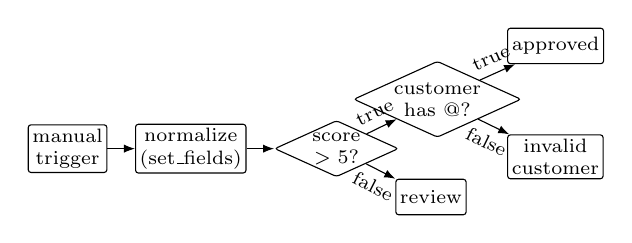
\begin{tikzpicture}[font=\scriptsize, node distance=2mm and 3.5mm,
  n/.style={draw, rounded corners=1pt, minimum height=4.5mm, inner sep=1.5pt, align=center},
  c/.style={n, diamond, aspect=2.2, inner sep=0.3pt},
  arr/.style={-{Latex[length=1.4mm]}}]
\node[n] (t) {manual\\trigger};
\node[n, right=of t] (n) {normalize\\(set\_fields)};
\node[c, right=of n] (th) {score\\$>5$?};
\node[c, above right=of th] (kc) {customer\\has @?};
\node[n, below right=of th] (rv) {review};
\node[n, above right=of kc] (ap) {approved};
\node[n, below right=of kc] (inv) {invalid\\customer};
\draw[arr] (t)--(n); \draw[arr] (n)--(th);
\draw[arr] (th)-- node[above,sloped]{true}(kc); \draw[arr] (th)-- node[below,sloped]{false}(rv);
\draw[arr] (kc)-- node[above,sloped]{true}(ap); \draw[arr] (kc)-- node[below,sloped]{false}(inv);
\end{tikzpicture}
\caption{Seven-node branching workflow used for the latency and throughput experiments.}
\label{fig:lat}
\end{figure}

\begin{table}[!htbp]
\centering
\caption{End-to-End Latency of the Seven-Node Workflow (\LATn{} Sequential Runs)}
\label{tab:lat}
\small
\begin{tabular}{L{3.3cm} r r r r}
\toprule
\textbf{Measure} & \textbf{Median} & \textbf{Mean} & \textbf{p95} & \textbf{Max} \\
\midrule
End-to-end wall time (ms) & 259.6 & 260.6 & 290.2 & 295.6 \\
Recorded step time, sum per run (ms) & 7.0 & 6.6 & 11.0 & 16.0 \\
\quad step: trigger (ms, n=50) & 2.00 & 2.02 & 4.00 & 7.00 \\
\quad step: normalize (ms, n=50) & 1.50 & 1.60 & 3.00 & 7.00 \\
\quad step: threshold (ms, n=50) & 1.00 & 1.20 & 2.00 & 3.00 \\
\quad step: known\_customer (ms, n=25) & 1.00 & 1.36 & 2.00 & 3.00 \\
\quad step: approved (ms, n=17) & 1.00 & 1.35 & 2.20 & 3.00 \\
\quad step: invalid\_customer (ms, n=8) & 1.00 & 1.00 & 2.00 & 2.00 \\
\quad step: review (ms, n=25) & 1.00 & 0.88 & 2.00 & 2.00 \\
\bottomrule

\end{tabular}
\end{table}

\subsection{Throughput and Worker Concurrency}
To measure how the queue behaves under a burst, the worker was stopped, \THRn{} runs of the same workflow were queued (\THRenq{} s of API time), and a worker was started with concurrency 1, 4 and 8 in turn. The makespan is taken from the database records, not the client clock: it is the interval from the earliest recorded step start to the latest recorded step finish across the \THRn{} runs, so it measures the worker and API draining the queue. Table~\ref{tab:thr} shows the results. Throughput rises from concurrency 1 to 4 and falls slightly at 8, which is consistent with the single API process and database being the shared resource: each run makes eight to ten step reports plus a claim and a completion call, so the API handles roughly ten requests per run, and more worker tasks only add contention once the API is saturated. All \THRn{} runs succeeded at every level. That no run is claimed by two workers is the property of the \texttt{SKIP LOCKED} claim; it is covered by the backend's concurrent-claim test, which passed in the suite run reported in Table~\ref{tab:impl}, rather than by this experiment.

\begin{table}[!htbp]
\centering
\caption{Burst of \THRn{} Queued Runs Drained by One Worker}
\label{tab:thr}
\small
\begin{tabular}{r r r r}
\toprule
\textbf{Concurrency} & \textbf{Makespan (s)} & \textbf{Runs/s} & \textbf{Succeeded} \\
\midrule
1 & 1.40 & 71.3 & 100/100 \\
4 & 0.56 & 178.5 & 100/100 \\
8 & 0.63 & 158.6 & 100/100 \\
\bottomrule

\end{tabular}
\end{table}

\subsection{Replay from a Chosen Step}
A nine-node chain (trigger followed by eight set-fields nodes) was run \REPreps{} times; after each run the harness replayed it from its fifth action, the sixth node, with an edited input. Table~\ref{tab:rep} shows that each replay copied \REPcopy{} upstream steps from the parent without executing them (they carry no start time) and executed \REPexec{}, exactly the chosen node and its three descendants, and that the replay's wall time is correspondingly lower than the full run's. Every replay recorded kind \texttt{replay} and the parent's identifier, and the replayed node received the overridden input.

\begin{table}[!htbp]
\centering
\caption{Replay of a Nine-Node Chain from Its Sixth Node (\REPreps{} Repetitions)}
\label{tab:rep}
\small
\begin{tabular}{L{3.6cm} r r}
\toprule
\textbf{Measure} & \textbf{Full run} & \textbf{Replay} \\
\midrule
Steps copied from parent & 0 & 5 \\
Steps executed & 9 & 4 \\
Wall time, median (ms) & 281.6 & 228.8 \\
Wall time, p95 (ms) & 308.0 & 256.9 \\
\bottomrule

\end{tabular}
\end{table}

\subsection{Technical SEO Audit Workflow}
The workflow of Fig.~\ref{fig:seo}, in its final form (a webhook trigger, an HTTP fetch with a declared user agent, a title condition and two verdict nodes), was activated and invoked once per target through the webhook endpoint. Table~\ref{tab:seo} lists each target, the HTTP status seen by the fetch node, the number of attempts the substrate recorded, and the verdict. Three behaviours of the substrate shape the results. First, the HTTP node treats any non-2xx response as a failed step, so a 404 or a 301 ends the run as \emph{failed} with the status in the step error and in the attempt record; the audit therefore reads the status from the attempt rather than from a condition, and the first version of the workflow, which branched on the status code, was simplified accordingly. Second, redirects are not followed, so a moved page is reported as 301 rather than as the page it points to, which is the correct behaviour for an audit. Third, the flaky target, which answers 500 twice and then 200, is reported as a pass with three recorded attempts, which distinguishes an unstable server from a broken page without any workflow logic. The \texttt{robots.txt} and sitemap targets are reachable but are not HTML, so the title rule reports them as missing a title; a real audit needs a second condition on the response's content type before the title check, which the existing nodes can express. Among the public pages, three passed; one answered 301 to the request as sent, which is a finding about that site's canonical host rather than an error of the platform; and one home page exceeded the HTTP node's 256~KiB response cap, so its fetch failed with that reason recorded, a limit discussed below.

\begin{table}[!htbp]
\centering
\caption{Technical SEO Audit Workflow: One Run per Target}
\label{tab:seo}
\scriptsize
\begin{tabular}{L{3.0cm} r r r L{1.4cm}}
\toprule
\textbf{Target} & \textbf{HTTP} & \textbf{Attempts} & \textbf{Fetch ms} & \textbf{Verdict} \\
\midrule
mock/ok & 200 & 1 & 13 & pass \\
mock/notitle & 200 & 1 & 10 & missing\_title \\
mock/missing & 404 & 1 & 2 & fetch\_failed \\
mock/moved & 301 & 1 & 5 & fetch\_failed \\
mock/flaky (500,500,200) & 200 & 3 & 765 & pass \\
mock/robots.txt & 200 & 1 & 6 & missing\_title \\
mock/sitemap.xml & 200 & 1 & 5 & missing\_title \\
example.com & 200 & 1 & 60 & pass \\
iana.org & 200 & 1 & 62 & pass \\
python.org & 200 & 1 & 118 & pass \\
en.wikipedia.org/wiki/Main\_Page & 200 & 1 & 305 & fetch\_failed \\
rust-lang.org & 301 & 1 & 38 & fetch\_failed \\
\bottomrule

\end{tabular}
\end{table}

\subsection{Fault Injection: Worker Killed During a Side Effect}
The property that most separates n9n from the reviewed frameworks is what happens when a worker dies in the middle of an action. Three single-action workflows were run against a mock endpoint that answers after eight seconds; in each case the harness waited until the action's step was recorded as \emph{running}, killed the worker with \texttt{SIGKILL}, and started a fresh worker half a second later. The fresh worker can only claim the run after the 60-second lease expires. Table~\ref{tab:fault} gives the outcome of each case. A GET is idempotent, so the run is re-queued, the step is executed a second time (attempt 2) and the run succeeds. A POST without an idempotency key is not safe to repeat, so the run is marked \emph{uncertain} with the reason recorded and is never retried by the platform. A POST with an idempotency key is re-queued and succeeds like the GET. The uncertain verdict was recorded \FAULTrecover{} s after the lease expired, at the fresh worker's next claim; the two recoverable runs finished about eight seconds later still, the time taken to execute the slow call a second time. Recovery time is therefore the lease length plus the action's own duration.

\begin{table}[!htbp]
\centering
\caption{Recovery After the Worker Is Killed Mid-Action (60 s Lease)}
\label{tab:fault}
\scriptsize
\begin{tabular}{L{2.2cm} L{1.4cm} r L{2.6cm}}
\toprule
\textbf{Interrupted action} & \textbf{Final status} & \textbf{s after kill} & \textbf{Step record} \\
\midrule
GET (idempotent by method) & \emph{succeeded} & 68.2 & call: succeeded, attempt 2 \\
POST, no idempotency key & \emph{uncertain} & 60.3 & call: running, attempt 1; lease expired during non-idempotent action \\
POST with idempotency key & \emph{succeeded} & 68.4 & call: succeeded, attempt 2 \\
\bottomrule

\end{tabular}
\end{table}

\subsection{Discussion}
The measurements support three claims about the substrate. It is cheap: the worker spends single-digit milliseconds on a seven-node graph, and end-to-end latency is set by polling and reporting, both of which are tunable. It is durable and replayable: every step, branch, skip and HTTP attempt is in the database, a run can be resumed from its records after a crash, and a finished run can be replayed from any node with reuse of upstream outputs. And it is honest about side effects: an interrupted non-idempotent action is surfaced as \emph{uncertain} rather than silently repeated or silently dropped. These are the properties Section~V found missing in the reviewed agent frameworks, and they are exactly the properties an agent node will inherit by being an ordinary step.

The measurements also expose limits. Throughput is bounded by the single API process and the chatty step protocol; a multi-replica deployment was not tested. The lease is fixed at 60 seconds, so recovery from a crash takes at least that long. The HTTP node's treatment of non-2xx responses as failures is right for integrations but means an audit workflow cannot branch on status inside the graph, and its 256~KiB response cap, which protects the step store, stopped the fetch of one large public page; a configuration option to pass non-2xx responses through as data, and a body-truncation mode for audits that only need the head of a page, are two small, clearly useful changes identified by this experiment.
\section{Limitations and Threats to Validity}
\begin{enumerate}
\item \textbf{Only the substrate is evaluated.} The builder, the explainer and the agent node are specified, feature-flagged and planned, but no model was called in this paper. Nothing here measures the quality, cost or reliability of an agentic decision.
\item \textbf{Single machine, single trial per configuration.} Latency and replay figures come from \LATn{} and \REPreps{} repetitions on one laptop; throughput and fault cases were run once per configuration. No confidence intervals are reported, and the absolute numbers will differ on other hardware and under container networking.
\item \textbf{Synthetic workflows.} The graphs contain set-fields and condition nodes whose work is trivial, so the measurements characterise the engine, not realistic action latency. The SEO targets were a local mock and five public pages fetched once.
\item \textbf{The SEO layer is a workflow, not a product.} The audit shows that technical checks can be expressed and recorded with the existing nodes; it does not implement crawling, scoring, or the content assessment that the agent node is meant to provide.
\item \textbf{Review coverage.} Twenty-two works were selected by relevance, not by a systematic search; venues were cited from the arXiv record where the publisher page was not checked.
\item \textbf{Not checked.} Multi-replica operation, the Flutter and mobile test suites, the Gmail trigger path, and behaviour under database failover were not exercised for this paper.
\end{enumerate}

\section{Evaluation Plan for the Agentic and SEO Layers}
The substrate measurements fix the baseline against which the remaining layers will be judged. The plan below uses metrics that the substrate already records, so each can be computed from the database without new instrumentation.
\begin{itemize}
\item \textbf{Builder validity rate:} fraction of generated graphs that pass the publish validator in round 1, 2 and 3, on a fixed set of natural-language requests covering every node type; failures are classified by validator message.
\item \textbf{Builder correctness:} fraction of validated graphs whose test run on a model-suggested sample input produces the expected leaf verdict, judged by a person against the request.
\item \textbf{Explainer agreement:} for a corpus of failed and uncertain runs with known causes, fraction where the likely cause matches, and confirmation that the enforced \texttt{safe\_to\_retry} rule is never contradicted in the stored response.
\item \textbf{Reliability over repeats:} pass\^{}k \cite{yao2024taubench} for builder and explainer over $k=5$ identical requests, since a single success says little about a stochastic component.
\item \textbf{Cost and latency per decision:} input and output tokens from the usage log, and wall time per request, against the per-user limit.
\item \textbf{Data policy:} the redaction test suite plus an audit that no outgoing request body contains a known secret from a seeded workflow.
\item \textbf{Agent node under faults:} repeat the fault-injection experiment with an agent node that calls a POST tool, confirming that an interrupted agent step is marked \emph{uncertain} and that its reasoning trace up to the kill is preserved in the step record.
\item \textbf{SEO audit at scale:} run the audit workflow over a sitemap of at least 500 URLs through the schedule trigger, reporting precision and recall of the title and status checks against a crawler baseline, attempts per URL, and the p95 per-URL time.
\item \textbf{Content assessment:} for a labelled set of pages and target queries, agreement between the agent node's relevance verdict and human raters, reported separately from the deterministic checks so that model error cannot hide behind them.
\end{itemize}

\section{Conclusion}
The reviewed literature gives workflow designers a rich set of patterns for making a model reason, call tools and cooperate with other models, and a consistent warning from every realistic benchmark that such agents remain unreliable. What it lacks is the systems layer beneath those patterns: a durable, replayable, side-effect-aware record of execution into which agentic decisions can be inserted without amplifying their failures. n9n is built around that layer. Its deterministic substrate, implemented in Go and Rust on PostgreSQL, validates workflows as acyclic single-trigger graphs, snapshots them immutably, executes them under leases with per-step and per-attempt records, replays them from any node, and classifies an interrupted non-idempotent action as uncertain rather than repeating it. On a local deployment the substrate ran a seven-node workflow in a median of \LATmedian{} ms end to end, drained \THRn{} queued runs at up to \THRbest{} runs/s, reused \REPcopy{} of nine steps on replay, expressed a technical SEO audit with existing nodes, and recovered correctly from a worker killed mid-action in all three fault cases. The agentic layer, a prompt-to-workflow builder with a validate-and-repair loop and a failure explainer whose retry verdict is enforced in code, is specified and feature-flagged but not yet measured, as is the content side of the SEO layer; Section~X gives the plan for both. The contribution of this paper is therefore the argument, the design and the measured substrate; the agentic claims remain to be earned by the experiments that the substrate now makes possible.

\begin{thebibliography}{99}
\bibitem{yao2023react} S. Yao, J. Zhao, D. Yu, N. Du, I. Shafran, K. Narasimhan, and Y. Cao, ``ReAct: Synergizing reasoning and acting in language models,'' in \emph{Proc. Int. Conf. Learning Representations (ICLR)}, 2023, arXiv:2210.03629.
\bibitem{schick2023toolformer} T. Schick, J. Dwivedi-Yu, R. Dess\`{i}, R. Raileanu, M. Lomeli, L. Zettlemoyer, N. Cancedda, and T. Scialom, ``Toolformer: Language models can teach themselves to use tools,'' 2023, arXiv:2302.04761.
\bibitem{wu2023autogen} Q. Wu, G. Bansal, J. Zhang, Y. Wu, B. Li, E. Zhu, L. Jiang, X. Zhang, S. Zhang, J. Liu, A. H. Awadallah, R. W. White, D. Burger, and C. Wang, ``AutoGen: Enabling next-gen LLM applications via multi-agent conversation,'' 2023, arXiv:2308.08155.
\bibitem{shinn2023reflexion} N. Shinn, F. Cassano, E. Berman, A. Gopinath, K. Narasimhan, and S. Yao, ``Reflexion: Language agents with verbal reinforcement learning,'' in \emph{Advances in Neural Information Processing Systems 36 (NeurIPS)}, 2023, arXiv:2303.11366.
\bibitem{wang2023plansolve} L. Wang, W. Xu, Y. Lan, Z. Hu, Y. Lan, R. K.-W. Lee, and E.-P. Lim, ``Plan-and-solve prompting: Improving zero-shot chain-of-thought reasoning by large language models,'' in \emph{Proc. 61st Annu. Meeting Assoc. Comput. Linguistics (ACL)}, 2023, arXiv:2305.04091.
\bibitem{yao2023tot} S. Yao, D. Yu, J. Zhao, I. Shafran, T. L. Griffiths, Y. Cao, and K. Narasimhan, ``Tree of thoughts: Deliberate problem solving with large language models,'' in \emph{Advances in Neural Information Processing Systems 36 (NeurIPS)}, 2023, arXiv:2305.10601.
\bibitem{wang2023voyager} G. Wang, Y. Xie, Y. Jiang, A. Mandlekar, C. Xiao, Y. Zhu, L. Fan, and A. Anandkumar, ``Voyager: An open-ended embodied agent with large language models,'' 2023, arXiv:2305.16291.
\bibitem{zhou2024webarena} S. Zhou, F. F. Xu, H. Zhu, X. Zhou, R. Lo, A. Sridhar, X. Cheng, T. Ou, Y. Bisk, D. Fried, U. Alon, and G. Neubig, ``WebArena: A realistic web environment for building autonomous agents,'' in \emph{Proc. Int. Conf. Learning Representations (ICLR)}, 2024, arXiv:2307.13854.
\bibitem{liu2024agentbench} X. Liu, H. Yu, H. Zhang, Y. Xu, X. Lei, H. Lai, Y. Gu, H. Ding, K. Men, K. Yang, S. Zhang, X. Deng, A. Zeng, Z. Du, C. Zhang, S. Shen, T. Zhang, Y. Su, H. Sun, M. Huang, Y. Dong, and J. Tang, ``AgentBench: Evaluating LLMs as agents,'' in \emph{Proc. Int. Conf. Learning Representations (ICLR)}, 2024, arXiv:2308.03688.
\bibitem{mialon2023gaia} G. Mialon, C. Fourrier, C. Swift, T. Wolf, Y. LeCun, and T. Scialom, ``GAIA: A benchmark for general AI assistants,'' 2023, arXiv:2311.12983.
\bibitem{press2023selfask} O. Press, M. Zhang, S. Min, L. Schmidt, N. A. Smith, and M. Lewis, ``Measuring and narrowing the compositionality gap in language models,'' in \emph{Findings of the Assoc. Comput. Linguistics: EMNLP}, 2023, arXiv:2210.03350.
\bibitem{wang2024codeact} X. Wang, Y. Chen, L. Yuan, Y. Zhang, Y. Li, H. Peng, and H. Ji, ``Executable code actions elicit better LLM agents,'' in \emph{Proc. 41st Int. Conf. Machine Learning (ICML)}, 2024, arXiv:2402.01030.
\bibitem{patil2023gorilla} S. G. Patil, T. Zhang, X. Wang, and J. E. Gonzalez, ``Gorilla: Large language model connected with massive APIs,'' 2023, arXiv:2305.15334.
\bibitem{li2023camel} G. Li, H. A. A. K. Hammoud, H. Itani, D. Khizbullin, and B. Ghanem, ``CAMEL: Communicative agents for `mind' exploration of large language model society,'' in \emph{Advances in Neural Information Processing Systems 36 (NeurIPS)}, 2023, arXiv:2303.17760.
\bibitem{hong2023metagpt} S. Hong, M. Zhuge, J. Chen, X. Zheng, Y. Cheng, C. Zhang, J. Wang, Z. Wang, S. K. S. Yau, Z. Lin, L. Zhou, C. Ran, L. Xiao, C. Wu, and J. Schmidhuber, ``MetaGPT: Meta programming for a multi-agent collaborative framework,'' 2023, arXiv:2308.00352.
\bibitem{shen2023hugginggpt} Y. Shen, K. Song, X. Tan, D. Li, W. Lu, and Y. Zhuang, ``HuggingGPT: Solving AI tasks with ChatGPT and its friends in Hugging Face,'' 2023, arXiv:2303.17580.
\bibitem{yao2024taubench} S. Yao, N. Shinn, P. Razavi, and K. Narasimhan, ``$\tau$-bench: A benchmark for tool-agent-user interaction in real-world domains,'' 2024, arXiv:2406.12045.
\bibitem{yang2024sweagent} J. Yang, C. E. Jimenez, A. Wettig, K. Lieret, S. Yao, K. Narasimhan, and O. Press, ``SWE-agent: Agent-computer interfaces enable automated software engineering,'' 2024, arXiv:2405.15793.
\bibitem{aggarwal2024geo} P. Aggarwal, V. Murahari, T. Rajpurohit, A. Kalyan, K. Narasimhan, and A. Deshpande, ``GEO: Generative engine optimization,'' in \emph{Proc. 30th ACM SIGKDD Conf. Knowledge Discovery and Data Mining (KDD)}, 2024, arXiv:2311.09735.
\bibitem{wang2024survey} L. Wang, C. Ma, X. Feng, Z. Zhang, H. Yang, J. Zhang, Z. Chen, J. Tang, X. Chen, Y. Lin, W. X. Zhao, Z. Wei, and J.-R. Wen, ``A survey on large language model based autonomous agents,'' \emph{Frontiers of Computer Science}, 2024, doi:10.1007/s11704-024-40231-1, arXiv:2308.11432.
\bibitem{xi2023rise} Z. Xi, W. Chen, X. Guo, W. He, Y. Ding, B. Hong, M. Zhang, J. Wang, S. Jin, E. Zhou, R. Zheng, X. Fan, X. Wang, L. Xiong, Y. Zhou, W. Wang, C. Jiang, Y. Zou, X. Liu, Z. Yin, S. Dou, R. Weng, W. Cheng, Q. Zhang, W. Qin, Y. Zheng, X. Qiu, X. Huang, and T. Gui, ``The rise and potential of large language model based agents: A survey,'' 2023, arXiv:2309.07864.
\bibitem{masterman2024landscape} T. Masterman, S. Besen, M. Sawtell, and A. Chao, ``The landscape of emerging AI agent architectures for reasoning, planning, and tool calling: A survey,'' 2024, arXiv:2404.11584.
\bibitem{n8n} n8n GmbH, ``n8n: Workflow automation documentation,'' \url{https://docs.n8n.io/}, accessed 2026-10-23.
\bibitem{langgraph} LangChain, Inc., ``LangGraph documentation,'' \url{https://langchain-ai.github.io/langgraph/}, accessed 2026-10-23.
\end{thebibliography}

\end{document}
